\documentclass{article}


% to compile a camera-ready version, add the [final] option, e.g.:
\usepackage[final]{neurips}

% to avoid loading the natbib package, add option nonatbib:
    % \usepackage[nonatbib]{neurips_2019}

\usepackage[utf8]{inputenc} 	% allow utf-8 input
\usepackage[T1]{fontenc}    		% use 8-bit T1 fonts
\usepackage{hyperref}       		% hyperlinks
\usepackage{url}            		% simple URL typesetting
\usepackage{booktabs}       		% professional-quality tables
\usepackage{amsfonts}       		% blackboard math symbols
\usepackage{nicefrac}       		% compact symbols for 1/2, etc.
\usepackage{microtype}      		% microtypography
%\usepackage{breqn}			% dmath
\usepackage{listings}
\usepackage{amsmath}     		% multiline
\usepackage{graphicx}
\usepackage{xepersian}
\usepackage{graphicx}



\settextfont{XB Niloofar.ttf}

\title{پاسخ تمرین سری ۱ }




\author{%
  محمدرضا عزیزی\\
  ۹۸۱۳۱۰۲۲ \\
  دانشکده مهندسی کامپیوتر\\
  دانشگاه صنعتی امیرکبیر (پلی‌تکنیک تهران)\\
  \texttt{mrazizi@aut.ac.ir} \\
}


\renewcommand{\baselinestretch}{1.5} 

\begin{document}


\begin{minipage}{0.1\textwidth}% adapt widths of minipages to your needs

\includegraphics[width=1.1cm]{aut_logo.png}
\end{minipage}%
\hfill%
\begin{minipage}{0.9\textwidth}\raggedleft
دانشگاه صنعتی امیرکبیر (پلی‌تکنیک تهران)\\
شبکه‌های عصبی (بهار ۱۳۹۹)\\
\end{minipage}
% \end{}


\makepertitle




% 1
\section{
راهکاری برای پیش‌پردازش داده‌ها
}

داده‌ها با استفاده از کتابخانه pandas بارگذاری کرده و از آن‌جایی که ستون‌های داده‌ها نام ندارد، ابتدا با توجه به توضیحات دیتاست، یک لیست برای نام ستون‌ها تعریف کرده و این نام‌ها را به ستون‌های دیتافریم بارگذاری شده اضافه می‌کنیم. لیست این نام‌ها به ترتیب برابر است با:

\begin{latin}
\begin{lstlisting}
["age", "workclass", "fnlwgt", "education", "education-num", 
"marital-status", "occupation", "relationship", "race", "sex", 
"capital-gain", "capital-loss", "hours-per-week", "native-country", "label"]
\end{lstlisting}
\end{latin}

ستون آخر که مربوط به برچسب داده‌است با با نام label نام‌گذاری کرده‌ایم. \\


سپس یک دیکشنری تعریف می‌کنیم که هر دوتایی کلید/مقدار آن، خود یک دیکشنری است. برای مثال به ازای کلید label، دیکشنری زیر را داریم:

\begin{latin}
\begin{lstlisting}
'label': {'<=50K':0, '>50K': 1}
\end{lstlisting}
\end{latin}

به ازای تمامی مقادیر تمامی ستون‌هایی که مقدار عددی ندارند، این دیکشنری را تعریف کرده و به هر مقدار اسمی، یک عدد نسبت می‌دهیم. این اعداد از برای هر متغیر از ۰ شروع شده و یک واحد یک واحد افزایش می‌یابد. 

در نهایت با استفاده از تابع replace از کتابخانه pandas، طبق دیکشنری تعریف شده، مقادیر اسمی را به مقادیر عددی تبدیل می‌کنیم.






% add page break after each section
\let\oldsection\section
\renewcommand\section{\clearpage\oldsection}



%%%%%%%%%%%%%%%%%%%%%%%%%%%%%%%%%%%%%%%%%%%%%%%%%%


% 2
\section{
بارگذاری داده‌ها و انجام پیش‌پردازش
}

\begin{center}
	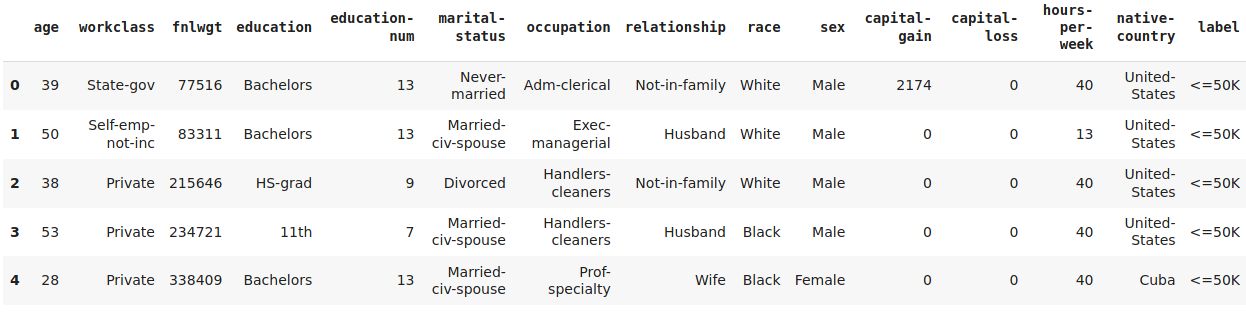
\includegraphics[scale=0.35]{df.png} 
\end{center}    


\begin{center}
	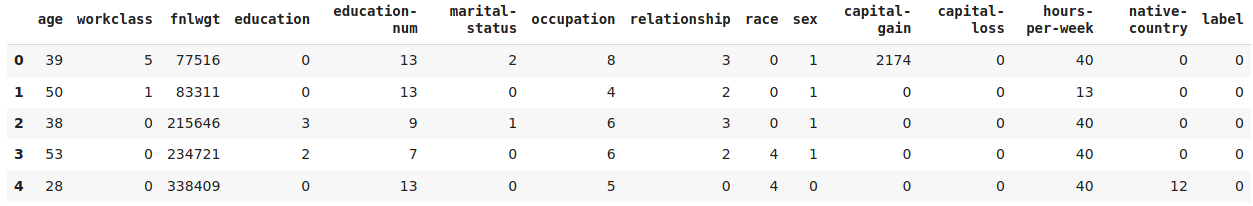
\includegraphics[scale=0.35]{df_numeric.png} 
\end{center}    


%%%%%%%%%%%%%%%%%%%%%%%%%%%%%%%%%%%%%%%%%%%%%%%%%%

%\section*{منابع}

\medskip

\small
\LTR 
\latin



\end{document}
